% ----------------------------------------------------------------
% Haupt-Dokument  ************************************************
%-----------------------------------------------------------------
%
% Autor:   Prof. Dr.-Ing. Dirk Benyoucef
% Version: V3.1
% Letzte �nderung : 28.09.2011
%
%-----------------------------------------------------------------
% Optionen des KOMA-Script Paket
%---------------------------------
\documentclass[11pt,                        % Schriftgr��e
               fleqn,                       % Gleichungen linksb�ndig
               halfparskip,                 %
               a4paper,                     % Papierformat A4
               headsepline,                 % einzeichnen einer Linie unter die Kopfzeile
               idxtotoc,                    % Aufnahme des Indexverzeichnis in das Inhaltsverzeichnis
               bibtotoc,                    % Aufnahme des Literaturverzeichnis in das Inhaltsverzeichnis
               liststotoc,
               bibtotocnumbered,            % Nummerierung des Literaturverzeichnis
               pointlessnumbers,            % Bei den Abschnittsnummern wird kein
                                            % Abschlie�ender Punkt gesetzt
               DIV15,                       % Andere Seitenaufteilung
               BCOR1.0cm,                   % Rand zum Binden
               openbib,						% Erzeugt Abs�tze im Literaturverzeichnis
               ngerman,
               ]{scrbook}
%-----------------------------------------------------------------
% Einbinden verschiedener n�tzlicher Pakete
%---------------------------------
\usepackage[ansinew]{inputenc}  % Erm�glicht die Verwendung von Umlaute
                                % und Sonderzeichen: 'ansinew'  f�r Windows
                                % 'latin1' f�r Linux
\usepackage[T1]{fontenc}        % 8-Bit-Fonts erleichtern die Trennung bei Umlauten
\usepackage[ngerman]{babel}     % deutschsprachige Anpassung; deutsche Trennmuster
\usepackage{varioref}
\usepackage{xcolor}             % Farbige Darstellung von W�rtern
\usepackage{framed}
\usepackage{graphicx}           % erm�glicht das Einbinden von Grafikdateien
\usepackage[sf,bf,SF,hang]{subfigure}   % Mehere Bilden in ein Abbildung
\usepackage[sf]{caption}        % Unterschrift in ein Abbildung
\usepackage{here}               % Bilder sollen beim Argument H an Ort und Stelle erscheinen
\usepackage{array}              % F�r komplexe Tabellen
%\usepackage{tabularx}           % Tabellen mit automatischer Berechnung der Spaltenbreite
\usepackage{booktabs}           % Tabellen
\usepackage{longtable}          % Erlaubt Tabellen �ber mehrere Seiten
\usepackage{multirow}           % F�r die Tabellen um mehrere Spalten zusammenzufassen
\usepackage{eurosym}            % Eurosymbol
\usepackage{url}                % Verwenden von URLs
\urlstyle{tt}
\usepackage[geometry]{ifsym}    % F�r Symbole
\usepackage[intlimits,sumlimits]{amsmath} % erweiterte Formeln, Optionen
                                % erm�glichen die Grenzen oberhalb und
                                % unterhalb zu setzen
\usepackage{amssymb}            % blackboard Buchstaben (z.B. Symbol f�r komplexe Zahlen IC)
\usepackage{theorem}            % Em�glicht die Definition von eigenen Umgebungen
\usepackage[amssymb,thickqspace]{SIunits}   % Vereinfacht den Umgang mit Einheiten
\usepackage{icomma}           % setzt das Komma bei Zahlen richtig (besonders bei mathematische Formeln)
\usepackage[pdfpagelabels,
            bookmarksnumbered=true,
            bookmarksopen=true,
            bookmarksopenlevel=1,
			pdftitle={ xxx},
			pdfauthor={ xxx },
			pdfsubject={Anleitung},
            pdfstartview=FitV,
			plainpages=false]{hyperref}
\usepackage{pdfpages}            % Mehrseitige PDFs einbinden
\usepackage[babel]{csquotes}
\usepackage{listings}
\usepackage{makeidx}
\usepackage{fancybox} 	% Boxen definieren und verorten
\usepackage{svn-multi}

\svnid{$Id: Ausarbeitung.tex 169 2011-09-28 14:22:43Z dbenyoucef $}


% Auswahl einer Schrift
\usepackage{cmbright}
%-----------------------------------------------------------------
% Einbinden einiger selbst definierten Makros
%---------------------------------
%
% Einige n�tzliche Makros f�r die Verwendung in Texten
%------------------------------------------------------
%
% Autor:   Dirk Benyoucef
% Version: V1.6
% Letzte �nderung : 55.02.2008
%

% Classe KOMA
%\renewcommand*{\capfont}{\captionfont}
%\renewcommand*{\caplabelfont}{\captionlabelfont}
\renewcommand{\figurename}{Bild}
\renewcommand{\tablename}{Tabelle}


% Umdefinition der Symbole f�r item
\renewcommand{\labelitemiii}{\FilledSmallSquare}
\renewcommand{\labelitemi}{\FilledSmallTriangleRight}
\renewcommand{\labelitemii}{\FilledSmallDiamondshape}

% Laborname
\newcommand{\DCSP}{\emph{Digital Communications \& Signal Processing }}

% Boxen definieren
\theoremheaderfont{\normalfont\bfseries}
\theoremstyle{break}
\theorembodyfont{\slshape}

\newtheorem{satzenv}{Anforderungen}[chapter]

\definecolor{boxgray}{gray}{0.9}

\newenvironment{graubox}{%
  \setlength{\fboxsep}{10pt}%
  \def\FrameCommand{\fcolorbox{black}{boxgray}}%
  \MakeFramed {\advance\hsize-30pt \FrameRestore}}%
 {\endMakeFramed}

\newenvironment{inhalt}%
{%
  \begin{graubox}
  \begin{satzenv}
}{%
  \end{satzenv}
  \end{graubox}
}

\newenvironment{grau_verbatim}%
{%
  \begin{graubox}
  \begin{verbatim}
}{%
  \end{verbatim}
  \end{graubox}
}


% Real- Imagin�rteil
\newcommand{\real}[1]{\operatorname{Re}{\left\{ #1 \right\}}}
\newcommand{\imag}[1]{\operatorname{Im}{\left\{ #1 \right\}}}

% Spezielle Befehle f�r OFDM
\newcommand{\Comment}[1]{}
\newcommand{\complex}[1]{\underline{#1}}
\newcommand{\dft}[1]{\operatorname{DFT}\left\{ #1 \right\}}
\newcommand{\idft}[1]{\operatorname{IDFT}\left\{ #1 \right\}}

\newcommand{\domega}{e^{j 2 \pi f T}}
\newcommand{\aOmega}{e^{j \Omega}}
\newcommand{\vOmega}{\Omega}

%
% STANDARDISIERUNG einiger SYMBOLE
%

% Mengenbuchstaben
%
\newcommand{\mm}[1]{\ensuremath{\mathbb{#1}}}
\newcommand{\mc}{\mm{C}}            % komplexe Zahlen
\newcommand{\mn}{\mm{N}}            % nat�rliche Zahlen
\newcommand{\mg}{\mm{G}}
\newcommand{\mi}{\mm{I}}
\newcommand{\mq}{\mm{Q}}
\newcommand{\mr}{\mm{R}}            % reelle Zahlen
\newcommand{\mw}{\mm{W}}
\newcommand{\mz}{\mm{Z}}            % ganze Zahlen
\newcommand{\rz}{{\mathbb R}}       % reelle Zahlen
\newcommand{\cz}{{\mathbb C}}       % komplexe Zahlen
\newcommand{\zz}{{\mathbb Z}}       % ganze Zahlen
\newcommand{\nz}{{\mathbb N}}       % nat�rliche Zahlen
\newcommand{\Nnull}{{\mathbb N}_0}  % nat�rliche Zahlen ohne die Null

\newcommand{\ma}{\mathcal{A}}            % Menge von A
\newcommand{\mb}{\mathcal{B}}            % Menge von B
\newcommand{\mt}{\mathcal{T}}
\newcommand{\mx}{\mathcal{X}}

% Einige Normen
\newcommand{\norm} [1]{\left\| #1 \right\|}
\newcommand{\lnorm}[1]{\left\| #1 \right\|_{l^2}}
\newcommand{\Lnorm}[1]{\left\| #1 \right\|_{L^2}}
\newcommand{\wnorm}[1]{\left\| #1 \right\|_{\mathrm W}}

% Skalarprodukte
\newcommand{\skalar} [2]{\left\langle #1, #2\right\rangle}
\newcommand{\lskalar}[2]{\left\langle #1, #2\right\rangle_{l^2}}
\newcommand{\Lskalar}[2]{\left\langle #1, #2\right\rangle_{L^2}}

% Erwartungswert
\newcommand{\erw}[1]{\mathcal{E}{\left\{#1\right\}}}
\newcommand{\var}[1]{\operatorname{var}\left\{#1\right\}}

% Vektoralebra
\newcommand{\rot}{\operatorname{rot}}
\newcommand{\divergenz}{\operatorname{div}}
\newcommand{\grad}{\operatorname{grad}}

% Neue Signale oder Operatoren
\newcommand{\dif}{\operatorname{d \!}}
\newcommand{\rect}{\operatorname{rect}}
\newcommand{\erfc}{\operatorname{erfc}}
\newcommand{\erf}{\operatorname{erf}}
\newcommand{\si}{\operatorname{si}}
\newcommand{\Si}{\operatorname{Si}}
\newcommand{\adj}{\operatorname{adj}}
\newcommand{\sign}[1]{\operatorname{sign}\left\{ #1 \right\}}
\newcommand{\spur}[1]{\operatorname{spur}\left\{ #1 \right\}}
\newcommand{\diag}[1]{\operatorname{diag}\left\{ #1 \right\}}
\newcommand{\Per}{\operatorname{Per}}
\newcommand{\Min}{\operatorname{Min}}


% Transformationen
\newcommand{\trafo}[1]{\mathcal{T}{\left\{#1\right\}}}
\newcommand{\four}[1]{\mathcal{F}{\left\{#1\right\}}}
\newcommand{\fourdft}[1]{\mathcal{F}_{DFT}{\left\{#1\right\}}}
\newcommand{\invfour}[1]{\mathcal{F}^{-1}{\left\{#1\right\}}}
\newcommand{\invfourdft}[1]{\mathcal{F}^{-1}_{DFT}{\left\{#1\right\}}}
\newcommand{\stft}[1]{\mathcal{F}{_{STFT}\left\{#1\right\}}}
\newcommand{\ztrafo}[1]{\mathcal{Z}{\left\{#1\right\}}}
\newcommand{\invztrafo}[1]{\mathcal{Z}^{-1}{\left\{#1\right\}}}
\newcommand{\hilbert}[1]{\mathcal{H}\left\{ #1 \right\}}
\newcommand{\hilbertinv}[1]{\mathcal{H}^{-1}\left\{#1 \right\}}
\newcommand{\stftmert}[1]{\mathcal{F}_{#1}^\gamma(\omega,\tau)}
\newcommand{\fourmert}[1]{\mathcal{F}_{#1}(\omega,\tau)}
\newcommand{\wave}[1]{\mathcal{W}{\left\{#1\right\}}}
\newcommand{\wavep}[1]{\mathcal{W}{_{WP}\left\{#1\right\}}}
\newcommand{\spec}[1]{S_{#1}(\omega,\tau)}


% Korrespondenzzeichen
\newcommand{\korresp}{\mbox{\setlength{\unitlength}{0.1em}%
                            \begin{picture}(34,10)%
                              \put(10,3){\circle{4}}%
                              \put(12,3){\line(1,0){11}}%
                              \put(24,3){\circle*{4}}%
                            \end{picture}%
                           }%
                     }%
\newcommand{\invkorresp}{\mbox{\setlength{\unitlength}{0.1em}%
                            \begin{picture}(34,10)%
                              \put(10,3){\circle*{4}}%
                              \put(11,3){\line(1,0){11}}%
                              \put(24,3){\circle{4}}%
                            \end{picture}%
                           }%
                     }%
\newcommand{\rotkorresp}{\mbox{\setlength{\unitlength}{0.1em}%
                            \begin{picture}(10,30)%
                              \put(6,8){\circle{4}}%
                              \put(6,10){\line(0,1){11}}%
                              \put(6,22){\circle*{4}}%
                            \end{picture}%
                           }%
                     }%
\newcommand{\rotinvkorresp}{\mbox{\setlength{\unitlength}{0.1em}%
                            \begin{picture}(10,30)%
                              \put(6,8){\circle*{4}}%
                              \put(6,9){\line(0,1){11}}%
                              \put(6,22){\circle{4}}%
                            \end{picture}%
                           }%
                     }%

% Matrix
\newcommand{\mat}[1]{{\mathbf{#1}}}
\newcommand{\dimension}[1]{\operatorname{dim}\left\{ #1 \right\}}


% Integral- und Summengrenzen ober- und unterhalb setzen
\newcommand{\intl}{\int\limits}
\newcommand{\suml}{\sum\limits}
\newcommand{\prodl}{\prod\limits}



% Darstellung eines Bruch mit einem Schr�gstrich
% Makro \nicefrac
%\newcommand{\nicefrac}[2]{\leavevmode\kern.1em\raise.5ex
%                          \hbox{\the \scriptfont0 #1}\kern
%                          -.1em / \kern-.15em\lower.25ex
%                          \hbox{\the \scriptfont0 #2} }

% Rahmen von Formeln
\newcommand{\rahmen}[1]{\boxed{\hspace{0.5cm}\begin{array}{c}#1\end{array}\hspace{0.5cm}}}
               % Sammlung von Abk�rzungen f�r Mathematiksymbolen
                                % (ben�tigt die Pakete amssymb und theorem)
\lstset{basicstyle=\sffamily,language=[Latex]Tex,frame=tb,numbers=left, numberstyle=\tiny, emphstyle=\color{red}, columns=fullflexible, backgroundcolor=\color{boxgray}}

\renewcommand{\labelitemiii}{\FilledSmallSquare}
\renewcommand{\labelitemi}{\FilledSmallTriangleRight}
\renewcommand{\labelitemii}{\FilledSmallDiamondshape}


% Auszufuehrende Befehle  ------------------------------------------------
\makeindex

% TITEL
\newcommand{\SEAT}{
\emph{Smart Metering: Disaggregation von Endverbrauchern }}
\newcommand{\SEA}{\emph{SmartMeter }}


%#################################################################
% Titelseite
% ----------------------------------------------------------------
% Einen Titel ausw�hlen
%\titlehead{\vspace{-2cm}
\includegraphics[height=15mm]{Bilder/Logo/DCSP_Lab_v1_1_grau.pdf}
           \hfill 
\includegraphics[height=20mm]{Bilder/Logo/Logo_HFU_rz_4c.pdf}\\
            \textsf{Hochschule Furtwangen}\\
            \textsf{Digital Communication \& Signal Processing Lab}\\
            \textsf{Prof. Dr.-Ing. Dirk Benyoucef}}

\subject{\textsf{Master Thesis}}
\title{Titel}
\author{Names des Studenten}
\date{\today}

\publishers{
    \begin{minipage}{\textwidth}
        \vskip 6cm
         {\normalsize }
         \begin{tabular}{ll}
            Betreuender Hochschullehrer: & Prof. Dr.-Ing. Dirk Benyoucef\tabularnewline
            Betreuender Mitarbeiter:& [Your tutor]\tabularnewline
            Tag der Anmeldung:& 01.03.2008 \tabularnewline
            Tag der Abgabe:   & 30.09.2008\tabularnewline
        \end{tabular}
        {\normalsize }
        \end{minipage}
    }
\extratitle{} 
%\titlehead{\vspace{-2cm}
\includegraphics[height=15mm]{Bilder/Logo/DCSP_Lab_v1_1_grau.pdf}
           \hfill 
\includegraphics[height=20mm]{Bilder/Logo/Logo_HFU_rz_4c.pdf}\\
            \textsf{Hochschule Furtwangen}\\
            \textsf{Digital Communication \& Signal Processing Lab}\\
            \textsf{Prof. Dr.-Ing. Dirk Benyoucef}}

\subject{\textsf{Bachelor Thesis}}
\title{Titel}
\author{Names des Studenten}
\date{\today}

\publishers{
    \begin{minipage}{\textwidth}
        \vskip 6cm
         {\normalsize }
         \begin{tabular}{ll}
            Betreuender Hochschullehrer: & Prof. Dr.-Ing. Dirk Benyoucef\tabularnewline
            Betreuender Mitarbeiter:& [Your tutor]\tabularnewline
            Tag der Anmeldung:& 01.03.2008 \tabularnewline
            Tag der Abgabe:   & 30.07.2008\tabularnewline
        \end{tabular}
        {\normalsize }
        \end{minipage}
    }
\extratitle{} 
\titlehead{\vspace{-2cm}
           \hfill 
\includegraphics[height=20mm]{Bilder/Logo/Logo_HFU_rz_4c.pdf}\\
            \textsf{}\\
            \textsf{}\\
            \textsf{}}

\subject{\textsf{WPV C\# \& Design Patterns}}      % Art der Arbeit
\title{Live Tuner}
\author{Alexander Baitinger, Tobias Grimm}
\date{\today}

\publishers{
    \begin{minipage}{\textwidth}
        \vskip 6cm
         {\normalsize }
         \begin{tabular}{ll}
            Betreuer der Hochschule: & Prof. Dr. Gerd Unruh\tabularnewline
        \end{tabular}
        {\normalsize }
        \end{minipage}
    }
\extratitle{} 

%#################################################################
% Begin des Document
% ----------------------------------------------------------------
\begin{document}
 
    \fancyput*(-1.8cm,-26cm){			 % Titelzeile auf allen Seiten
    	\rotatebox{90}{
    		\color{gray}
    		\footnotesize
    		\sf{}
    	}
    }

    \pagenumbering{roman}
    \maketitle                        % Erzeugen der Titelseite und der Widmung
    \tableofcontents                  % Erzeugen des Inhaltsverzeichnisses

    \frontmatter
%    \chapter*{Kurzfassung}
\begin{graubox}

Das Ziel dieses Projekts besteht darin, ein neues Verfahren für die automatische Codegenerierung zu Untersuchen.

Es wird eine Simulink Library für optimalen Code erstellt.
Diese wird verwendet, um ein Simulink Modell für eine Feldorientierte Regelung einer Permanent magnetisierten Synchronmaschine aufzubauen, zu simulieren, und auf einen ti-Microcontroller zu übertragen.

In einem letzten Schritt werden die simulierten Werte mit realen Messgrößen verglichen.

\end{graubox}

\begin{graubox}

...(englisch)
\end{graubox}
%    \chapter*{Kurzfassung}
\begin{graubox}

Das Ziel dieses Projekts besteht darin, ein neues Verfahren f�r die automatische Codegenerierung zu untersuchen.

Es wird eine Simulink Library f�r optimalen Code erstellt.
Diese wird verwendet, um ein Simulink Modell f�r eine feldorientierte Regelung einer permanent magnetisierten Synchronmaschine aufzubauen, zu simulieren, und auf einen ti-Microcontroller zu �bertragen.

In einem letzten Schritt werden die simulierten Werte mit realen Messgr��en verglichen.
\end{graubox}

\begin{graubox}

The goal of this project is the examination of a new method for automatic code generation. 

A Simulink library for optimal code has been implemented, which is used to build a Simulink 
Model for a field-oriented control of a permanent magnetic synchronous machine, to simulate and to transfer it to a ti-microcontroller.
 
In a last step the simulated dates are compared with real measured values.

\end{graubox}		
    \chapter*{Personen des Projekts}

%---------------------------------------
\begin{table}[h]
  \sffamily
  \centering
  \small
  %\caption{Bearbeiter des Projektes}
  \label{tab:Personen}
  \begin{tabular}{m{4cm} m{3cm} m{8cm} }
    \toprule
    Name & Foto & E-Mail Adresse\\
   \midrule

      Alexander Baitinger      & 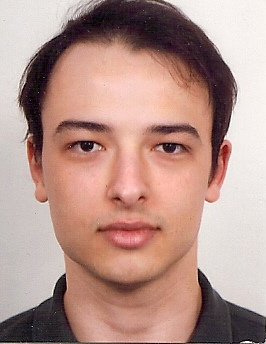
\includegraphics[width=3cm]{Bilder/Personen/Alexander_B.jpg} & alexander.baitinger@hs-furtwangen.de\\\\
   \cmidrule(lr){1-3}
      Tobias Grimm      & 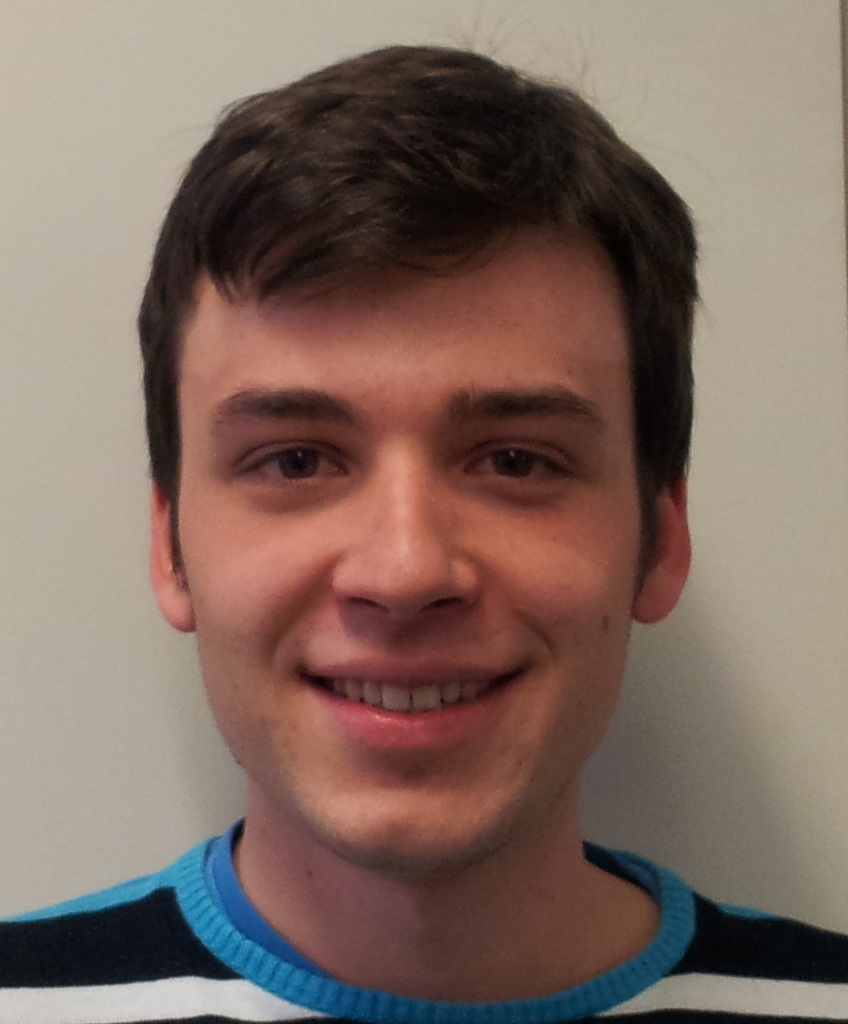
\includegraphics[width=3cm]{Bilder/Personen/Tobi_G.jpg} & tobias.grimm@hs-furtwangen.de\\
   \bottomrule
  \end{tabular}
\end{table}
    \cleardoublepage                  % zum Beenden der roman Seitennummerierung! \clearpage
    \pagenumbering{arabic}            % Seitennummerierung Hauptteil

    \cleardoublepage

    % Hauptteil
    \mainmatter

    %#################################################################
    % Kapitel
    % ----------------------------------------------------------------
    \chapter{Einleitung}

Das 6. Semester der Hochschule Furtwangen beinhaltet f�r den Studiengang Elektronik und Technische Informatik (ETI) die M�glichkeit durch Wahlpflicht Vorlesungen (WPVs) das gesamt Bild des angehenden Ingenieurs abzurunden.

Gerade f�r einen Elektrotechniker bietet es sich daher an, nicht nur die elektrotechnische Welt zu kennen, sondern auch die unz�hligen M�glichkeiten der Informatik kennen zu lernen, und diese in Kombination zu nutzen.

Aus diesem Gedanken heraus, ist die Idee entstanden ein Programm mit C\# zu entwickeln, welches den Arbeitsalltag eines Elektrotechnikers enorm erleichtern kann, indem regelungstechnische Auslegungen schnell und komfortabel durchgef�hrt werden k�nnen.

Um beide Welten sauber in Einklang bringen zu k�nnen wird auf der elektrotechnischen Seite auf die Regelungstechnik mit der Laplace-Transformation und die Z-Transformation zur�ck gegriffen und auf der Informatik Seite auf die Vorz�ge der Objektorientierten Programmiersprache C\# und die Verwendung von "`Design Patterns"'.

%---------------------------------------------------------
\section{Wichtiges �ber die Regelungstechnik}
\begin{description}

\item \textbf{Warum Regelungstechnik?}

In sehr vielen Anwendungen kommt es vor, dass man einen soll-Wert vorgibt, und diesen mit einem ist-Wert vergleicht und dann entscheidet was gemacht werden soll. Dieser Vorgang wird in der Regelungstechnik behandelt.

So kann man sich z.B. vorstellen, dass ein Motor auf eine gewisse soll-Drehzahl beschleunigt werden soll. Da die Drehzahl sich wegen der Tr�gheit der Masse des Motors nicht direkt auf die gew�nschte Drehzahl begibt, wird ein Regler eingesetzt. Dieser schaut sich den Soll-Ist Vergleich an und entscheidet dann, ob entweder \textit{mehr Drehmoment} oder \textit{weniger Drehmoment} aufgebracht werden muss, um den Motor auf die gew�nschte Drehzahl zu bringen.

\begin{figure}[H]
	\centering
  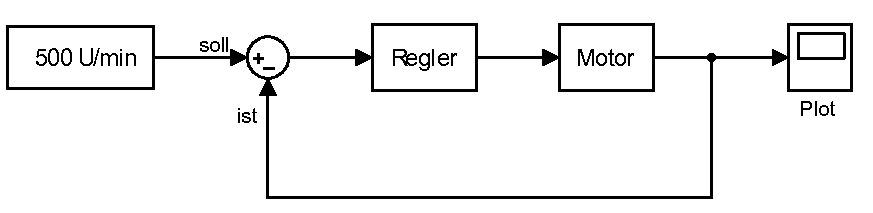
\includegraphics[width=1\textwidth]{Bilder3/Motor_Regelkreis.pdf}
	\caption{Beispiel Regelkreis f�r einen Motor}
	\label {Beispiel Regelkreis f�r einen Motor}
\end{figure}

In der Regelungstechnik werden nun verfahren untersucht, um diesen Regler ideal einzustellen, damit das zeitlich dynamische Verhalten eines Vorgangs ideal in den Griff gebracht werden kann.


\item \textbf{Was sind �bertragungsfunktion?}

Um dynamische Vorg�nge in der Physikalischen Welt Mathematisch beschreiben zu k�nnen werden in der Regel so genannte Differentialgleichungen eingesetzt.
Hierdurch kann z.B. das dynamische Verhalten eines Motors, einer elektronischen Schaltung, einer Temperatur, eines mechanischen Vorgangs, ... beschrieben werden.

Das eigentliche Problem besteht nun oft darin, dass das l�sen dieser Differentialgleichung sehr schwer ist. 
An dieser Stelle bietet die Laplace-Transformation einen eleganten Weg, um aus einer Differentialgleichung eine �bertragungsfunktion im Laplace-Bereich zu gewinnen.

Diese �bertragungsfunktion (Transferfunktion) bietet f�r unsere Zwecke entscheidende Vorteile:

\begin{itemize}
	\item \textit{Handhabung}
	
	Es ist wesentlich einfacher mit einer �bertragungsfunktion zu rechnen.
	\item \textit{Universell}
	
	Die Regelungstechnik ist f�r alle dynamischen Vorg�nge equivalent!
	\item \textit{Simulierbar}
	
	Durch Verwendung der Z-Transformation kann eine �bertragungsfunktion "`relativ"' einfach auf einem Computer Simuliert werden.
	\item \textit{Betrachtung als Block}
	
	Die einzelnen �bertragungsfunktionen f�r Regler, Motor, ... k�nnen als Bl�cke wie in Bild\vref{Beispiel Regelkreis f�r einen Motor} betrachtet werden.
\end{itemize}

\newpage
\item \textbf{Warum ein extra Software Tool?}

Die gesamte Regelungstechnik besteht zum gr��ten Teil aus Mathematik. Hier kann es sehr schnell passieren, dass man den �berblick verliert, da es einem schwer f�llt sich gewisse abstrakte Gebilde vorzustellen. 

Das hier entwickelte Software Tool m�chte genau an dieser Stelle ansetzen, dem Benutzer ein Gef�hl daf�r zu geben, wie die einzelnen abstrakten Gebilde zusammenh�ngen, und welchen Einfluss die einzelnen Parameter auf das dynamische Verhalten des Systems haben.

Dar�ber hinaus sind bereits verfahren hinterlegt, um einen Regler gut auszulegen, und diesen visuell in Echtzeit an die Bed�rfnisse des Ingenieurs nach tu tunen.
Aus diesem grund hat das neu entstandene Tool den Namen "`Live-Tuner"' erhalten.

\end{description}
%    \section{Systemkonzept (Adam Visy)}

In diesem Kapitel wird das Konzept erkl�rt, mit dem  das Problem aus der Aufgabenstellung gel�st wurde.
Die Abbildung \vref{fig:syskonzept} dient zur Veranschaulichung des L�sungswegs der gegebenen Aufgabenstellung. Der Kern des eingebetteten Systems besteht aus demPIC32MX795F512L der Firma Microchip, sowie aus einer auf das DCSP11 Board basierten Platine.

Bei der Bet�tigung des Tasters wechselt das System vom Ruhezustand in den normalen Betrieb. Hier k�nnen nun verschiedene Ausgaben �ber die Stroboskopuhr dargestellt werden. Die vom DCF77-Empfangsmodul ermittelte Uhrzeit wird bei Bedarf mit der internen Uhrzeit durch den RTCC synchronisiert und gegebenenfalls �ber die RGB LEDs ausgegeben. Die RGB LEDs werden �ber drei TLCs, die �ber einen I2C-Bus mit dem PIC kommunizieren, angesprochen. Eine weitere Ausgabem�glichkeit, f�r Wartungszwecke, stellt das Display dar. Der Summer erm�glicht eine akustische Ausgabe f�r zum Beispiel die Weckfunktion. Das Pendel wird von einem Gleichstrommotor der Firma Dunkermotoren bewegt. Die Drehzahl wird  analog vom Mikrocontroller vorgegeben. Die Position des Zeigers wird mithilfe eines, auf dem Pendel befindenden, Hallsensors festgestellt. �ber einen Photowiderstand wird die Umgebungslichtst�rke gemessen. So kann die Lichtst�rke der RGB-LEDs angepasst werden. Der Webserver soll �ber die Ethernetschnittstelle von au�en angesprochen werden. Der Webserver wird auf einer mit ebenfalls SPI-Bus angebundenen SD-Karte hinterlegt.

\begin{figure}[htbp]
	\centering
		\includegraphics[width=0.8\textwidth]{Bilder/syskonzept3.pdf}
	\caption{Blockschaltbild des Sysemkonzepts}
	\label{fig:syskonzept}
\end{figure}



    \chapter{Aufbau des Live Tuners}
\label {Aufbau des Live Tuners}
%%%%%%%%%%%%%%%%%%%%%%%%%%%%%%%%%%%%%%%%%%%%%Aufbau des Live Tuners%%%%%%%%%%%%%%%%%%%%%%%%%%%%%%%%%%%%%%%%
In diesem Kapitel wird der eigentliche Aufbau der Software des Live Tuners n�her beschrieben. Eine erste �bersicht bietet hier das UML-Klassendiagramm\vref{UML Klassendiagramm}.

\begin{figure}[H]
	\centering
  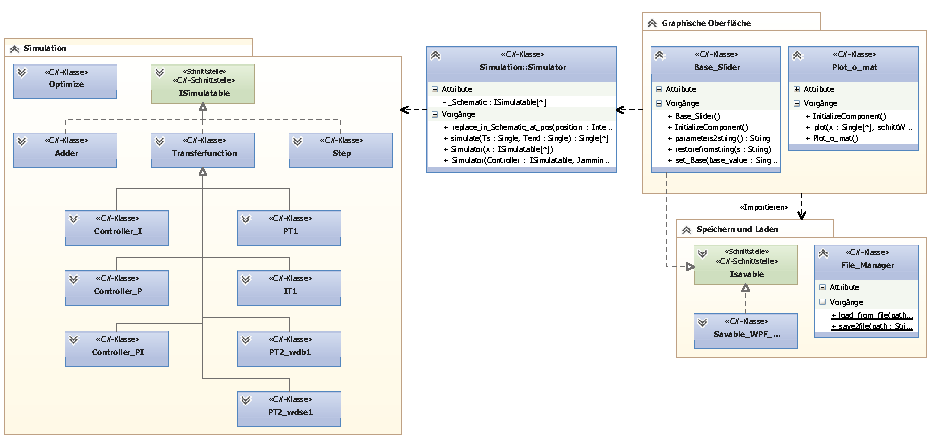
\includegraphics[width=1.1\textwidth]{Bilder3/UMLClassDiagram1.pdf}
	\caption{UML-Klassendiagramm}
	\label{UML Klassendiagramm}
\end{figure}

Wie leicht zu erkennen ist, baut sich der Live Tuner aus drei gro�en Komponenten auf:

\begin{itemize}
	\item \textit{Graphische Oberfl�che} \vref{Graphische Oberfl�che}
	\item \textit{Simulation} \vref{Simulation}
	\item \textit{Speichern und Laden} \vref{Speichern und Laden}
\end{itemize}

Diese drei Komponenten werden nun in diesem Kapitel n�her beleuchtet.

%%%%%%%%%%%%%%%%%%%%%%%%%%%%%%%%%%%%%%%%%%%%%Graphische Oberfl�che%%%%%%%%%%%%%%%%%%%%%%%%%%%%%%%%%%%%%%%%
\section{Graphische Oberfl�che}
\label {Graphische Oberfl�che}


\begin{description}
	 
		\item \textbf{Das Ziel}
		
Blablabla Benutzerfreundlich blablabla ... WPF der Hammer blablabla

\begin{figure}[H]
	\centering
  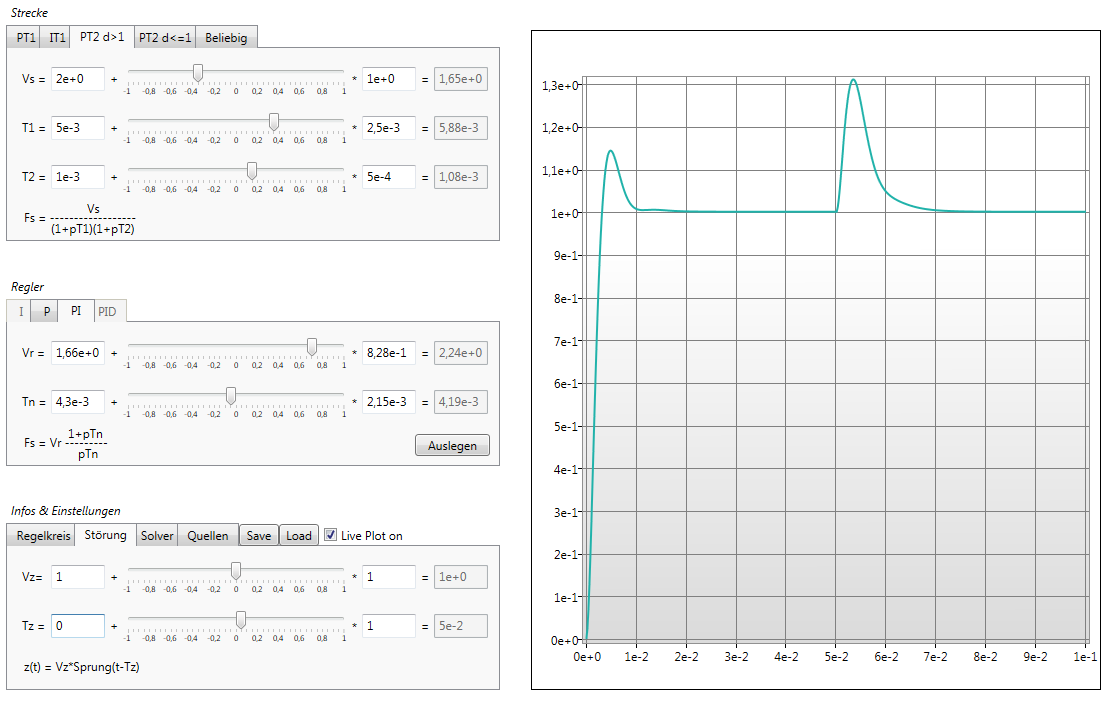
\includegraphics[width=1\textwidth]{Bilder3/Live_Tuner.png}
	\caption{Graphische Oberfl�che des Live Tuners}
	\label{Graphische Oberfl�che des Live Tuners}
\end{figure}

		\item \textbf{Live Plot}

Blablablablub

		\item \textbf{Strecke und Regler}		
				
Blablabla Verschiedene Strecken -> der passende Regler wird vorgeschlagen blablabla Auslegen geht nur wenn Strecke passt blablabla

		\item \textbf{Base Slider}	
		
Beschreiben warum er Base Slider hei�t + wie ist er aufgebaut (basis + slider*mult) + warum es so cool ist blablalba

		\item \textbf{Infos \& Einstellungen}
			
Beschreiben was man hier sieht bzw. machen kann ... verlinkung bei Solver zu Simulation ....				
			
\end{description}

\newpage 
%%%%%%%%%%%%%%%%%%%%%%%%%%%%%%%%%%%%%%%%%%%%%Simulation%%%%%%%%%%%%%%%%%%%%%%%%%%%%%%%%%%%%%%%%
\section{Simulation}
\label {Simulation}

Durch die komplette Simulation eines Regelkreises soll dem Benutzer graphisch gezeigt werden, wie gut sein aktueller Regler ausgelegt ist.
Ein allgemeiner Regelkreis besteht aus folgenden Komponenten:

\begin{figure}[H]
	\centering
  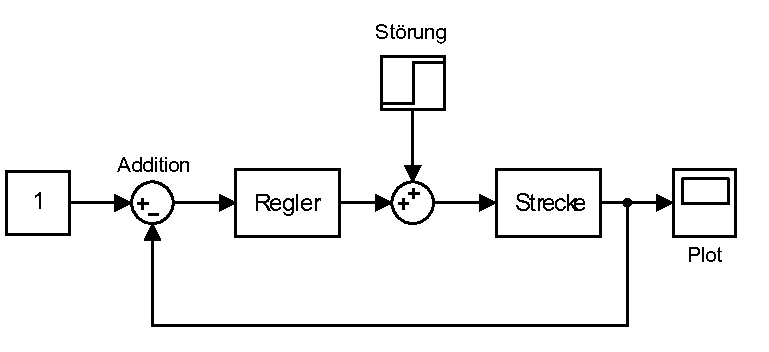
\includegraphics[width=1\textwidth]{Bilder3/Regelkreis.pdf}
	\caption{Allgemeiner Aufbau eines Regelkreises}
	\label{fig:Aufgabe11}
\end{figure}

\begin{itemize}
	\item \textit{Soll-Wert}
	
	Gew�nschter Wert, welcher erreicht werden soll.
	\item \textit{Vergleich Soll-Ist}
	
	Durch die Addition(+/-) wird ein Soll-Ist Vergleich gemacht, welcher zum Regler geht.
	\item \textit{Regler}
	
	Der Regler ist eine �bertragungsfunktion, und je nach Bedarf ein P-, I-, oder PI-Regler.
	\item \textit{St�rung}
	
	Durch die St�rung sollen m�gliche St�rfaktoren mit Simuliert werden.
	\item \textit{Strecke}	
	
	Die Strecke ist die �bertragungsfunktion des Physikalischen Systems (Motor, elektrische Schaltung,...)
	\item \textit{Plot}
	
	Der Plot beobachtet quasi die einzelnen Simulationsschritte und gibt diese graphisch aus.
\end{itemize}

Die Idee f�r die softwaretechnische Umsetzung einer Simulation besteht nun darin, dass jede einzelne Komponente des Regelkreises durch eine einzelne Klasse beschrieben wird.
Bei einer Simulation berechnet nun jeder Teilnehmer einen kleinen Zeitschritt und gibt das Ergebnis an den n�chsten Teilnehmer im Regelkreis weiter. Dies wird so oft wie erw�nscht wiederholt und am Schluss als Gesamtergebnis zur�ckgegeben.

\begin{description}

		\item \textbf{Die Problematik}

\begin{itemize}
	\item Die ganzen Berechnungen der Simulation eines Regelkreises sind sehr kompliziert, wie kann man es nach au�en vereinfachen, sodass man sich nicht hinein denken muss, wenn man dieses verwenden will?
	\item Die einzelnen Klassen im Regelkreis f�r Regler und Strecke k�nnen je nach Anwenderbedarf unterschiedlich sein! Wie k�nnen nun diese Klassen mit einander Kommunizieren, ohne sich direkt kennen zu m�ssen? 
\end{itemize}

				
		\item \textbf{L�sungsansatz}
		
Einen sehr guten L�sungsansatz bieten hier die Schablonen der Entwurfsmuster (Design Patterns). Hierbei handelt es sich um bew�hrte L�sungsschablonen f�r wiederkehrende Entwurfsprobleme in der Softwareentwicklung.

Um diese zwei Probleme zu behandeln wurden folgende zwei Entwurfsmuster ausgew�hlt:

\newpage				
\subsection{Fassade Entwurfsmuster}%%%%%%%%%%%%%%%%%%%%%%%%%%%%%%%%%%%%%%%%%%%%%%%%%%%%%%
\label{Fassade Entwurfsmuster}	

		\item \textbf{Beschreibung des Entwurfsmusters \cite{FDP:01}}
		
\textit{Wenn ein Subsystem viele technisch orientierte Klassen enth�lt, die selten von au�en verwendet werden, hilft es, eine Fassade zu verwenden. Die Fassade ist eine Klasse mit ausgew�hlten Methoden, die eine h�ufig ben�tigte Untermenge an Funktionalit�t des Subsystems umfasst. Sie delegiert die Funktionalit�t an andere Klassen des Subsystems und vereinfacht dadurch den Umgang mit dem Subsystem.}


		\item \textbf{Verwendung der Fassade}

Wie im Ausschnitt des UML-Diagramms\vref{UML Klassendiagramm2} gut zu erkennen ist, bildet die Klasse \textit{Simulator} eine Fassade in diesem Projekt. 
	
\begin{figure}[H]
	\centering
  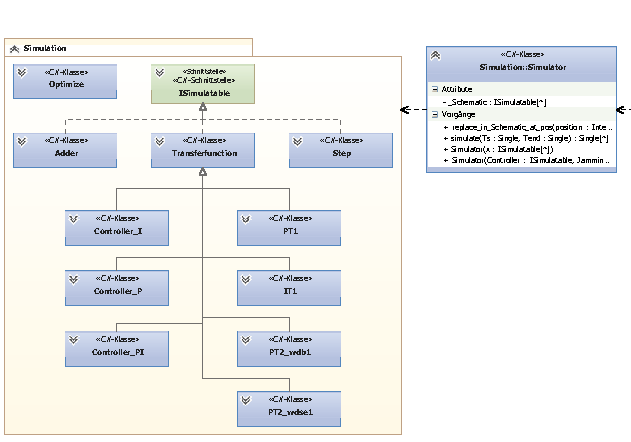
\includegraphics[width=1.1\textwidth]{Bilder3/UMLClassDiagram2.pdf}
	\caption{Klasse "`Simulator"' als Fassade}
	\label{UML Klassendiagramm2}
\end{figure}

Der \textit{Simulator} k�mmert sich um die komplette Verwaltung der einzelnen Klassen einer Simulation, vernetzt sie miteinander und leitet die einzelnen Berechnungen. Er merkt sich in einem Array von Objekten, welche das Interface ISimulatable implementieren, in welcher Reihenfolge die einzelnen Objekte bei einer Simulation aufgerufen werden m�ssen.

Durch diesen Einsatz wird die komplexit�t einer Simulation auf ein Minimum von zwei Funktionen herunter gebrochen:

\begin{itemize}
	\item \textit{simulate(Ts : Single, Tend : Single) : Single[*]}
	
	Simuliere den aktuellen Regelkreis mit den festen kleinen Zeitschritten Ts bis zur Endzeit Tend. Gebe das Ergebnis zur�ck.
	
	\item \textit{bool replace\_in\_Schematic\_at\_pos(int position, ISimulatable x)}
	
	Ersetze im Array an der Stelle \textit{position} das Objekt mit diesem. L�se die alten Vernetzungen und setze neue. (hierdurch k�nnen die Objete im Regelkreis vertauscht werden)
\end{itemize}
 
\subsection{Beobachter Entwurfsmuster}%%%%%%%%%%%%%%%%%%%%%%%%%%%%%%%%%%%%%%%%%%%%%%%%%%%%%%
\label{Beobachter Entwurfsmuster}	
		
		\item \textbf{Beschreibung des Entwurfsmusters \cite{BDP:01}}
		
\textit{Allgemein finden Beobachter-Muster Anwendung, wenn eine Abstraktion mehrere Aspekte hat, die von einem anderen Aspekt derselben Abstraktion abh�ngen, die �nderung eines Objekts �nderungen an anderen Objekten nach sich zieht oder ein Objekt andere Objekte benachrichtigen soll, ohne diese im Detail zu kennen.}	

		\item \textbf{Verwendung des Beobachter-Musters}

Dieses Muster bietet sich ideal f�r das zweite Problem an, da sich die einzelnen Objekte in einem Regelkreis nicht direkt kennen m�ssen, um sich gegenseitig benachrichtigen zu k�nnen.
Diese Benachrichtigungen sind immer dann erforderlich, wenn ein Objekt im Regelkreis einen Zeitschritt f�r sich berechnet hat. Ist die Berechnung fertig, so wird das Ergebnis an das Beobachtende Objekt weitergegeben.
Anschaulich bedeutet dies, dass alle Verbindungen im Regelkreis\vref{Benachrichtigungen in einem Regelkreis} solche Benachrichtigungen (events) sind.

\begin{figure}[H]
	\centering
  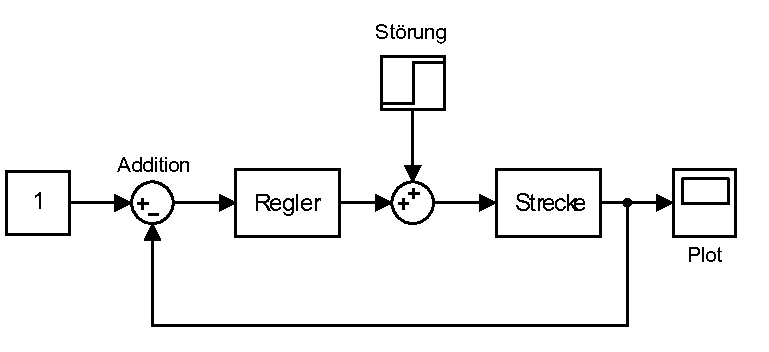
\includegraphics[width=1\textwidth]{Bilder3/Regelkreis.pdf}
	\caption{Benachrichtigungen in einem Regelkreis}
	\label{Benachrichtigungen in einem Regelkreis}
\end{figure}

\newpage

Hierdurch ist nun klar, wie das Interface aussehen muss, welches eine Klasse implementieren muss, um simulierbar zu sein:

\begin{figure}[H]
	\centering
  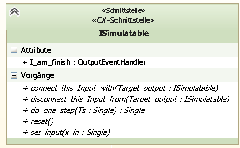
\includegraphics[width=0.5\textwidth]{Bilder3/Interface_IS.pdf}
	\caption{Interface f�r Simulation}
	\label{Interface f�r Simulation}
\end{figure}



\begin{itemize}
	\item \textit{event OutputEventHandler I\_am\_finish}
	
	Dieses event wird gefeuert, wenn eine Berechnung fertig ist.
	\item \textit{void set\_input(float x\_in)}
		
	Setze den Eingangswert f�r die Berechnung des n�chsten Zeitschrittes.
	\item \textit{float do\_one\_step(float Ts)}
		
	Berechne den Ausgangswert aus dem Eingangswert und feuere das Event I\_am\_finish.
	\item \textit{void reset()}	
	
	Leere den Speicher der Vergangenheit.
	
	\item \textit{void connect\_this\_Input\_with(ISimulatable Target\_output)}

	Beobachte den Ausgang des anderen Objektes, indem du deinen Eingang mit diesem Ausgang verbindest.
	\item \textit{void disconnect\_this\_Input\_from(ISimulatable Target\_output)}
	
	L�se die Beobachtung auf.
\end{itemize}

Durch dieses Interface und die verwendung des Simulators kann nun der Regelkreis simuliert werden.
Im UML-Sequenzdiagramm\vref{UML Sequenzdiagramm} ist eine Benutzeranfrage an eine Simulation skizziert.
		
\begin{figure}[H]
	\centering
  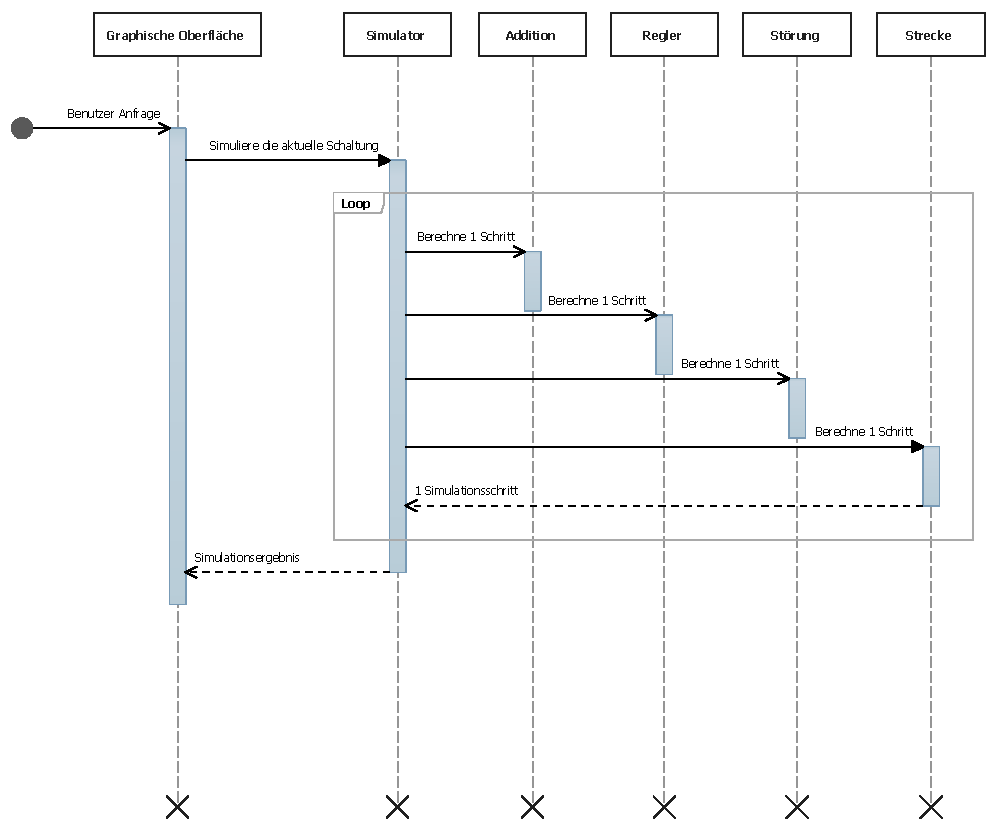
\includegraphics[width=1\textwidth]{Bilder3/UMLSequenceDiagram1.pdf}
	\caption{UML-Sequenzdiagramm f�r eine Simulationsanfrage}
	\label{UML Sequenzdiagramm}
\end{figure}

Wie deutlich zu erkennen ist, benutzt die Graphische Oberfl�che die Fassade des Simulators um eine Simulation zu starten.
Dieser ruft nach und nach die einzelnen Komponenten des Regelkreises dazu auf einen Zeitschritt zu berechnen. 
Wie klar zu erkennen ist, kennen sich die einzelnen Komponenten des Regelkreises nicht, sondern beobachten sich nur gegenseitig, um Informationen zu erhalten.

Haben alle Komponenten einen Zeitschritt berechnet, so wird die Schleife erneut durchlaufen bis die gew�nschte Anzahl an Simulationsschritten erreicht ist, und das gesamt Ergebnis an die Graphische Oberfl�che zur�ck gegeben wird.
				
\end{description}

\newpage
%%%%%%%%%%%%%%%%%%%%%%%%%%%%%%%%%%%%%%%%%%%%%%Speichern und Laden%%%%%%%%%%%%%%%%%%%%%%%%%%%%%%%%%%%%%%%%%%%%%%%%%%
\section{Speichern und Laden}
\label {Speichern und Laden}
\begin{description}
		
		\item \textbf{Die Motivation}
		
blablablub viel Zeit investiert alles weg. ..... Anderen Leuten Schicken .... Archivieren ....
				
		\item \textbf{Umsetzung}

Interfave beschreiben ekl�ren ,.....
Fale Manager beschreiben ... warum ist er so vielseitig einsetzbar ...
		
\end{description}
%    \chapter{Zusammenfassung}
In diesem Abschnitt ist zu beschreiben, welche Arbeiten durchgef�hrt wurden. D.h. die eigene Leistung ist unter Hinweis auf die dabei verwendeten Methoden und Vorgehensweisen hier darzustellen. Dabei ist eine Einordnung der Ergebnisse in das allgemeine Problemumfeld vorzunehmen, das in Einleitung und Stand der Technik zur Sprache kam. Sie sollten hier auf die vorhergehenden Kapitel verweisen, um dem Leser der quer liest, die M�glichkeit zu geben, die Details anzusehen ({\LaTeX } \verb+\ref{...}+).

%---------------------------------------------------------
\section{ToDo}
An dieser Stelle sind die Arbeiten aufzuf�hren, die noch zwingend durchgef�hrt werden sollen. Punkte aus dem Pflichtenheft, die optional waren und Aspekte, die sich aus dem Projekt neu ergeben haben.

%---------------------------------------------------------
\section{Ausblick}
Im Ausblick ist darzustellen, wie das Projekt weitergef�hrt werden kann. Dies kann auch einen konkreten Arbeitsplan enthalten.

%---------------------------------------------------------
\section{Fehlerliste}
In diesem Abschnitt ist anzugeben, ob Fehler in der Arbeit enthalten sind, die nicht mehr beseitigt werde konnten. F�r eine Weiterf�hrung der Arbeit ist dies sehr wichtig.

    \chapter{Zusammenfassung}

... blablabla alles Top 

%---------------------------------------------------------
\section{Ausblick}

Der Simulator kann alles Simulieren -> nichtleare komponenten einf�hren, ... als basis f�r gr��ere Schaltungssimulation....
File Manager kann in Beliebigen Projekten verwendet werden....

    %#################################################################
    % Anhang
    % ----------------------------------------------------------------
 %   \appendix
   \chapter{Quellenverzeichnis}

Bei der Einarbeitung in das Projekt und der eigentlichen Programmierung, wurden folgende Dokumente verwendet.

\begin{description}
	 
\item \textbf{Fachliteratur:}
				
\begin{itemize}
	\item C\# Quick Reference    -    Apress
	\item Auf der Faehrte von C\#    -    Springer
	\item C\# 3.0 Design Patterns    -    O'Reilly 
\end{itemize}

\item \textbf{Skripte:}
				
\begin{itemize}
	\item Regelungstechnik    -    Prof. Dr. Konstantin Meyl
	\item Systemtheorie    -    Prof. Dr. Peter Strobach
\end{itemize}

\item \textbf{Internetseiten:}
				
\begin{itemize}
	\item http://msdn.microsoft.com/
	\item http://stackoverflow.com/
	\item http://de.wikipedia.org/wiki/Fassade\_(Entwurfsmuster)
	\item http://de.wikipedia.org/wiki/Beobachter\_(Entwurfsmuster)
	\item https://wpftoolkit.codeplex.com/
\end{itemize}

\end{description}
 %   \chapter{Erkl�rung der selbst�ndigen Anfertigung}

\begin{figure}[htbp]
	\centering
%		\includegraphics[angle=0,scale=0.4]{Bilder2/Selbstaend.png}
%	\caption{Sperrvermerk}
%	\label{fig:Sperrvermerk}
\end{figure}

%\begin{figure}[htbp]
%	\centering
%		\includegraphics[angle=0,scale=0.4]{Bilder2/Sperrvermerk.png}
%	\caption{Sperrvermerk}
%	\label{fig:Sperrvermerk}
%\end{figure}

 %   \chapter{Nomenklatur}
 %   \section{Abk�rzungen}
 %       \renewcommand\arraystretch{1.2}  % Multiplikationsfaktor f�r die
                                 % Zeilenumbr�che in der Tabelle
\begin{longtable}[t]{p{2.5cm} p{13cm}<{\raggedright}}
  A/D, D/A          & Analog/Digital bzw. Digital/Analog\\
  AKF               & Autokorrelationsfunktion\\
  AWGN              & additives, wei�es, Gau�sches Rauschen (additive white Gaussian noise)\\[2mm]

  BER               & Bitfehlerrate (bit error rate)\\[2mm]

  CDMA              & Code Division Multiple Access\\[2mm]

  DFT               & Discrete Fourier Transformation \\
  DMT               & Discrete Multi Ton\\[2mm]

  FDMA              & Frequency Division Multiple Access\\
  FDD               & Frequency Division Duplex\\
  FFT               & Fast Fourier Transformation \\[2mm]

  WMF               & Whitening Matched Filter\\[2mm]
\end{longtable}

 %   \section{Symbole und Formelzeichen}
 %       %\renewcommand\arraystretch{1.5}  % Multiplikationsfaktor f�r die
                                 % Zeilenumbr�che in der Tabelle
\begin{longtable}[t]{p{4cm} p{11.5cm}<{\raggedright}}

\multicolumn{2}{l}{\textbf{Konstante Gr��en}}\\
  $e$                         & Eulersche Zahl, $e \approx 2,71828183$\\
  $\pi$                       & Kreiszahl,    $\pi \approx 3.14159265$\\
  
\multicolumn{2}{l}{\textbf{Formelzeichen}}\\
  $R$                         & Widerstand\\
  $C$                         & Kapazit�t\\
  $L$                         & Induktivit�t\\
  $u$													& Spannung\\
  $i$                         & Stromst�rke\\
  $t$													& Zeit\\
  $f$                         & Frequenz\\
  $n$                         & Drehzahl\\
  $\omega$                    & Kreisfrequenz\\
  $\varphi$                   & Elektrischer Winkel\\
  $M$                         & Drehmoment\\
 
\multicolumn{2}{l}{\textbf{Einheiten}}\\
   V                         & Volt\\
   W           							 & Watt\\
  $\Omega$                   & Ohm\\
	 S                         & Siemens\\
   F                         & Farrad\\
	 H                         & Henry\\
   s                         & Sekunde\\
   m					    					 & Meter\\
   A											   & Ampere\\
   Hz                        & Hertz\\
	 N                         & Newton\\
   B                         & Byte (8 Bit)\\

  
  
\multicolumn{2}{l}{\textbf{Vors�tze}}\\
   n                         &$10^{-9}$\\
   $\mu$                    &$10^{-6}$\\
   m                         &$10^{-3}$\\
   k                         &$10^{3}$\\
   M                         &$10^{6}$\\
\multicolumn{2}{l}{\textbf{Funktionen}}\\
  $\ln$                        & Logarithmus Naturalis\\
  $\sin$                      & Sinus\\
  $\cos$                       & Kosinus\\
  $\tan$                       & Tangens\\
  sig                       & Sigmoid\\
\end{longtable}


    \bibliographystyle{Alphadin}    % Alphabetisch sortiertes Literaturverzeichnis mit
                                    % Einordnungsmarken aus Verfasser und
                                    % Erscheinungsjahrk�rzeln
%    \bibliography{Literaturstellen} % erzeuge Literaturverzeichnis
                                    % benutze Literaturdatenbank
                                    % Literaturstellen d.h. die Dateien diplom.bib

    % Abbildungs- und Tabellenverzeichnis
    \listoffigures
%    \listoftables
%    \renewcommand{\lstlistlistingname}{Listingverzeichnis}
%    \lstlistoflistings

    \printindex

\end{document} 